

%%% This LaTeX source document can be used as the basis for your technical
%%% report. Intentionally stripped and simplified
%%% and commands should be adjusted for your particular paper - title, 
%%% author, citations, equations, etc.
% % Citations/references are in report.bib 

\documentclass[conference,backref=page]{acmsiggraph}

\TOGonlineid{45678}
\TOGvolume{0}
\TOGnumber{0}
\TOGarticleDOI{1111111.2222222}
\TOGprojectURL{}
\TOGvideoURL{}
\TOGdataURL{}
\TOGcodeURL{}

% Include this so that citations show up in blue and the page information is included in the reference section
\hypersetup{
    colorlinks = true, 
    linkcolor = blue,
    anchorcolor = red,
    citecolor = blue, 
    filecolor = red, 
}


\title{Mesh Destruction\\
	   Design Document}

\author{Conner Weatherston \thanks{e-mail:40167111@live.napier.ac.uk} \\
Edinburgh Napier University\\
Physics-Based Animation (SET09119)}
\pdfauthor{Conner Weatherston}

\keywords{bounding volumes, rigid bodies, real-time, voronoi fracture}

\begin{document}

\teaser{
   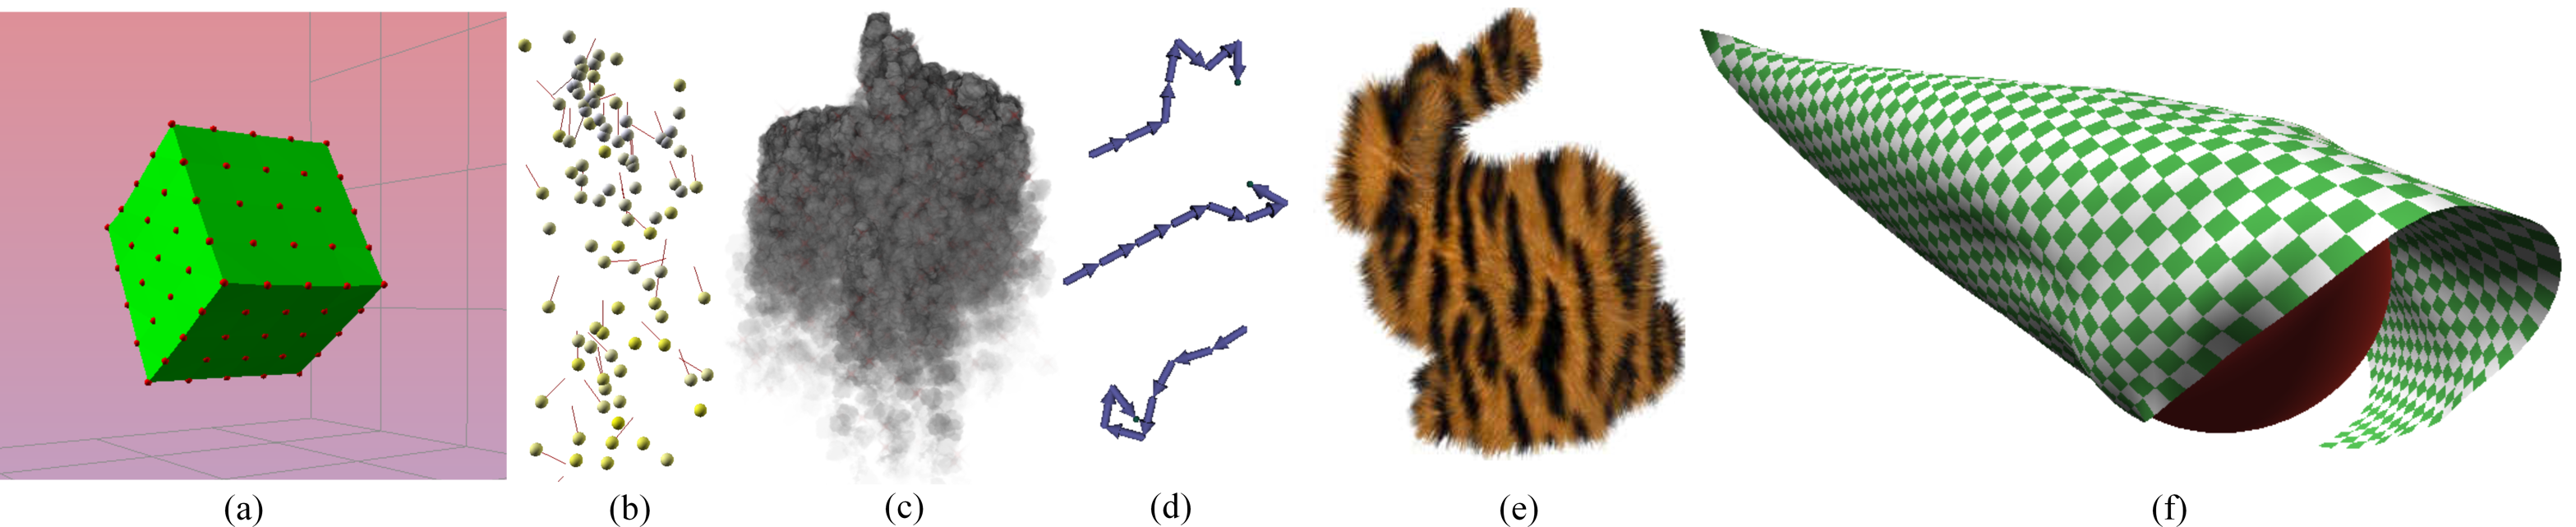
\includegraphics[height=1.5in]{images/sampleteaser}
   \caption{Place a teaser image at the top of your report to show key examples of your work (e.g., multiple screenshots of the different test situations) - Every figure should have a caption and a description.  For example, each figure is labelled and explained: (a) soft bodies, (b) particles, (c) inverse kinematics, (e) fur shells, and (f) position-based dynamics for cloth effects.}
   \label{fig:teaser}
 }

\maketitle

\raggedbottom

\begin{abstract}

In most physics based games, any destructible objects are normally loaded in with their fractured components on runtime. This physics simulation is looking at using a 3D implementation of voronoi diagrams to create fractures patterns. This technique is known as voronoi fracturing. When an appropriate collision has occurred then the model fragments should be created using the fragment lines as an guide to how the fragments are formed.


The abstract is typically a single paragraph.  The abstract is the first thing people read when they encounter your report; hence, it is crucial that it outlines all the important aspects of your report.  Make your abstract incredibly concise and clear.  You start with the problem and end with why your solution is interesting.  Briefly explain why your solution is valuable and how you have evaluated it.  Keep your abstract small.  Typically, the abstract should be approximately 100 words.

\end{abstract}



\keywordlist

%% Use this only if you're preparing a technical paper to be published in the 
%% ACM 'Transactions on Graphics' journal.

% \TOGlinkslist

% \copyrightspace


\section{Introduction}


\paragraph{What problem are you solving?}
The introduction sells your physics-based simulation effect.  It tells the reader about the problems and motivation.  It tells the reader about why it is important.  Your introduction should be five clear well defined paragraphs \cite{day2012write}.

I am solving the issue of me wanting a university degree so I have to do this physics simulation to pass.

In most games with destructible objects the fragments have been pre-calculated a loaded into the game and when the main object is destroyed it is replaced with the fragments instead. This simulation is looking at creating the fragments using the original model data. 



\paragraph{What is the motivation? (What's so interesting and important?)}
Explain why your simulation is important?  Why would you need it?  Where would it be used?
My motivation for this project is ... I had to do it for coursework.

\paragraph{Challenging \& Limitations}
Why is it hard? (e.g., why do naive approaches fail?)
There are several issues with tackling this problem. The two main ones are generating a voronoi diagram in 3 dimensions. This can be solved using Delauney triangulation. The second issue is performance, this is due to the creation of several objects when the model fractures. Hence optimisation will be a major part of this simulation to work effectively.


\paragraph{Our Work}
Why hasn't it been solved before or what are you doing differently? How does yours differ?
What's your approach?  How will you solve the problem?  Are their any specific limitations?


\paragraph{Starting examples:}
This report attempts to addresses the problem of the applicability of …. in ….. by considering …...  It surveys a number of answers to this question.  Our method offers a simplistic, robust, and reliable scheme.

This report attempts to introduce the reader to …… 
(Catch the readers attention, Anecdotes, Proverbs, Facts, Real-World Examples...)

The problem this report addresses is …..


\section{Related Work}
Refer to literature on the particular physics-based animation effect you want to synthesize (e.g., published articles, books, conference proceedings, web articles) provide a comprehensive review - and use the correct citation format, e.g., \cite{Sako00}. Although the theoretical and/or algorithmic details of the papers you will review may occasionally be beyond your current knowledge, you should be able to grasp the general principles of the techniques used and assess whether you are capable of developing similar techniques, more advanced techniques, or whether you would need to simplify these techniques. 



Related work should finish with a summary paragraph - emphasising the crucial similarities or differences between existing methods presented in the literature.  For example: (1) you might want to modify the technique to run on the GPU; (2) or you combine different techniques from different authors; (3) or you are simplifying the algorithm to make it run faster.

% SIMULATION
\section{Simulation}

\paragraph{Overview}
You will start with a brief overview of the core principles and mechanism behind your effect.  This should be reflected in your final implementation, so consider what you will actually be implementing. What components make up the effect and how are they connected.

How does your simulation work and what are the reasons it is important.  This is a decisive section to put together as it will help you in the rest of your physics-based animation development.

\paragraph{Detailed description}
Provide a more detailed description of how the simulation functions. Consider the following aspects of the simulation:
\begin{itemize}
\item {\bf Functionality}: Describe what your simulation does and the anticipated boundaries of its functionality.
 The simulation will have several objects in the scene that interact with each other. When a appropriate collision between two models has occurred. One of the models will shatter.
 
\item {\bf Method}: Present the theory underpinning your technique (Mathematical, physics or algorithmic principles) and the technique itself. You should be able to articulate a general algorithm at this stage.
\item {\bf Control/interactivity}: Describe the interactive how the simulation will be controlled
 This simulation will be interactive as the user can move one of the models around in the scene as well as being able to change the number of fragments a model can generate. 
\end{itemize}


















Pseudo code.
1. Sample points inside the model.
2. Generate Delaunay triangulation.
3. Obtain dual voronoi diagrams from Delaunay triagnulation.
4. For each voronoi cell in model. (Size is number of sample points).
		for each plane in cell.
				split model.



1. Sample points.
1.1 Get how many fragments are needed.
1.2 For(int i=0; i <numFragments; i++)
		1.2.1 change face ray starts on.
			1.2.2 end point is opposite face.
			 1.2.3 Find in/out point of ray.
			 1.2.4 for (samplesPerRay)
			    1.2.3 samples.add(point);
			    end for
			end for


3. Detect suitable collisions
\paragraph{Implementation}
At the design stage, you are not expected to provide information about the implementation, but you need to consider and reflect on the technical challenges that you will need to address. You also need to provide information about relevant technical aspects of your project. Please consider the following points:

\begin{itemize}
\item  {\bf Major Software Development Tasks} What are the major pieces of development to make the software work?  Identify the main tasks from the simulation design, particularly items you feel will be difficult to implement. 
\item {\bf Risks} What are the risks in your development?  Consider which pieces of functionality will be difficult to implement, and what are the options if you cannot achieve them.
\item {\bf External Libraries} Are you using any external libraries or resources to implement your simulation?  If you are using any libraries outside the ones developed in the practical sessions, these will need to be described here.
\end{itemize}

In your final report, this section will present the final implementation details. You should also reflect on the differences between the approach proposed in your design document and the final implementation.

% EVALUATION
\section{Testing and evaluation}
In this section of the {\bf Design document}, you should describe the tests that you are considering carrying out to test your evaluation and ensure that it works within its specified boundaries. In your {\bf Final report}, you will present the actual evaluation that you have carried out and reflect on its outcome. In particular, you may consider the actual performance of your simulation in relation to your initial goals. A comparison to relevant work would also be beneficial.

\section{Guidelines}
This section should be removed from your design report. Information provided here is to help you writing up your reports.

\begin{itemize}
\item Equations should be numbered and in the correct format, e.g., Equation \ref{eq:myequation} below:
\begin{equation} \label{eq:myequation}
 \sum_{j=1}^{z} j = \frac{z(z+1)}{2}
\end{equation}
\item Furthermore, if you include an equation, ensure you explain what each of the variables are (e.g., $F$ is force, $m$ is mass, and $a$ is the acceleration).
\item Don't using 'I' or 'Me'.
\item Each paragraph should be clear and focused, with multiple sentences that help make your point - avoid lots of single line paragraph sentence.
\item Make sure the citations are done using the correct formatting (i.e., .bib file and let LaTeX generate the references).
\item Every figure should have a caption, explaining what the picture is and what the reader should be looking at (i.e., what is important about the figure, what does it show)
\item A figure should also be referenced in the body of the main text (e.g., see Figure \ref{fig:teaser})
\item Equations should be numbered, and referenced in the text. Furthermore, ensure each of the variables in the equation are explained (i.e., don't use F=ma and not say what F, a, and m are)
\end{itemize}


\section{Conclusion and Future work}
The report should finish with a summary to give a brief overview of what the reader should remember most.  What was most important? The future work part only needs to be covered in your final report.


% \section*{Acknowledgements}


\bibliographystyle{acmsiggraph}
\bibliography{report}

\end{document}

